\section{Design and Implementation}
\label{sec:implementation}

This section discusses the implementation and design of \MP{}. To profile an allocator, \MP{} intercepts memory allocations/deallocations, memory-related system calls, and synchronizations. This also indicates that an allocator should utilize standard APIs in order for \MP{} to collect corresponding information. However, the Linux allocator utilizes the internal implementation of synchronizations by default. For the profiling purpose, it should be changed to invoke explicit POSIX-APIs instead. Fortunately, most allocators do not need any change or the recompilation.  \MP{} profiles the performance, memory overhead, scalability, and application friendliness, as discussed in different subsections. 

 %It also discusses some common issues, such as adapting to different allocators, and the performance issue of collecting data. 

\subsection{Profiling Performance Data}

\label{sec:performanceimplement}

\MP{} profiles the performance overhead of every memory management operation. Since an allocator typically has different execution paths for different scenarios (as discussed in Section~\ref{sec:allocator}), such as new or re-used allocations, small or big objects, \MP{} further collects the information for each scenario separately. The fine-grained data helps identify a particular design issue inside. For instance, DieHarder has a serious performance issue for deallocating small objects for \texttt{dedup}, with 744105 cycles and 2.8 cache misses for each deallocation. However, it has the similar number of cycles and deallocation runtime  for deallocating big objects. Given the fine-grained data, programmers could only focus on the deallocation path relating to small objects.

\MP{} collects the allocation data for small objects and large object separately, where small objects further include new and re-used allocation. For deallocation, \MP{} collects the deallocation data for small and big objects separately. \MP{} collects the average runtime of each allocation and deallocation with the RDTSC instruction,
%(Section~\ref{sec:pmu}), 
due to the performance and accuracy reason. Time stamps are taken before and after each operation, and then the difference between them is the runtime of an operation. 

\MP{} differentiates the types of an operation as follows. To differentiate small and big objects, \MP{} relies on a configuration file as further described in Section~\ref{sec:understandingallocators}. It is also important to differentiate between new and re-used allocations, since they typically have over $20\times$ performance difference on average. \MP{} uses a global hash map to assist this differentiation: every allocated object will be inserted into the global hash map in its allocation time, and will be kept in the table; If an allocation is found to be in the hash map, then this allocation is a re-used allocation. Otherwise, it is a new allocation.  


\MP{} also employs the PMUs to collect hardware events of each operation, such as cache misses, page faults, TLB misses, and instructions. These hardware data are  significant supplements for identifying an issue, given that \MP{} is a non-intrusive profiler that cannot know the implementation details of an allocator. Let us revisit the issue of DieHarder. DieHarder is found to have a large number of cycles for its deallocation. However, it is difficult to know the particular issue inside, if without more information. An unusual number of cache misses for each deallocation helps identify the design issue: DieHarder traverses all bags one by one to determine the original bag for an allocation, causing excessive number of cache misses. Similarly, \MP{} collects hardware events before and after each operation, and uses the difference of two counters as the number of events occurring inside an operation. 

\subsection{Profiling Memory Overhead}
\label{sec:profilingmemory}

For memory overhead, \MP{} reports the ratio of different types of memory overhead, such as internal fragmentation, memory blowup, and other memory overhead, and real memory usage. Therefore, programmers can pinpoint memory consumption clearly. We have described the concepts of different types of overhead in Section~\ref{sec:memoryconsumption}. However, it is challenging to collect corresponding data correctly and efficiently.


Conceptually, internal fragmentation is the difference between the size class and the requested size for a small object. However, if the difference is larger than a page, the internal fragmentation cannot be computed  with this method. We need to consider page allocation policy, where the OS only allocates a physical page if it is used. Based on this, internal fragmentation for such objects should be adjusted correspondingly: for a new allocation, the fragmentation will be difference between the end of the object and the end of its last page; For a re-used object, \MP{} should track the maximum pages of this object, and use the difference between the end of its last page and the end of the object as internal fragmentation. When an object is released, its internal fragmentation should be decremented. \MP{} utilizes the same hash map as described in Section~\ref{sec:performanceimplement} to track the maximum pages for each object. 

It is challenging to compute memory blowup correctly. By the definition of Section~\ref{sec:memoryconsumption}, a new allocation will be treated as memory blowup if there exist freed objects of this size class in the freelists of other threads. However, this definition does not specify whether memory blowup should be reduced upon deallocations, and what to do if such objects are subsequently re-allocated again. \MP{} computes memory blowup based on the following observation: \textit{all freed objects of a size class represent the upper bound for its memory blowup.} Then, \textit{the upper bound deducted by the size of recently-freed objects represents its memory blowup}. This definition is intuitive, since recently-freed objects do not belong to memory blowup, as they will exist anyway by necessity. Based on this definition, \MP{} further implements a practical method to compute the number of recent objects. The intuitive method simply utilizes a global counter to track recently-freed objects across each size class. This counter is incremented upon every deallocation, but will be decremented upon each allocation as long as the counter's value is greater than zero.


In addition, it is very expensive to frequently collect all data, when memory consumption reaches its maximum value. Therefore, \MP{} only updates this data periodically, when the total memory usage is increased by 1MB. Also, it is also very expensive to update all data using global counters, since this will cause significant cache contention. Therefore, \MP{} tracks most data using thread-local variables, then summarizes all data together when reaching the maximum memory consumption. \MP{} only uses global variables for the memory consumption and the counts of recently-freed objects. However, even with these two global variables, it is expensive to update them with the full synchronization or even atomic variables. Instead, \MP{} updates these variables without synchronization primitives or the use of atomic variables, which may lose some updates. However, based on our evaluation, \MP{} should still provide a reliable percentage for different types of memory overhead.  

%these data,  real memory usage is the amount of memory actually requested by the application, where real allocated memory is the sum of real memory usage and internal fragmentation due to size-class based allocation. For example, if an application requests the memory by \texttt{malloc(454)}, then real memory usage is incremented by $454$, but real allocated memory will be incremented by the size of its corresponding class size. For this example, total memory will be incremented by page size instead (e.g., 4096 bytes), provided that the page was previously unused. 



%\MP{} also collects different types of memory overhead, such as internal fragmentation, memory blowup, and others. It also collects the available memory and total memory consumption of each size class. The detailed data help programmers to pinpoint its memory overhead issue. For instance, if memory overhead mainly comes from the internal fragmentation, then the allocator should utilize more fine-grained size classes. If the memory overhead mainly comes from memory blowup, the allocator may require to adjust its synchronization frequency or take a more aggressive method for its synchronization~\citep{DBLP:conf/iwmm/LiLD19}. The memory overhead could be reduced with coalescence or splitting, if the major memory overhead comes from external fragmentation. 

%\MP{} typically records different counters upon each allocation and deallocation. For the performance reason, \MP{} typically maintains a per-thread counter in order to reduce the contention issue. The per-thread counters includes the number of allocations and deallocations for each size class, the number of bytes for internal fragmentation, and allocated objects for each size class. \MP{} utilizes a global hash table to track the status information for each object, Therefore, \MP{} could adjust the internal fragmentation upon each deallocation. 



% \MP{} reports other memory overhead as a summarized value, including external fragmentation, metadata overhead, and explicitly skipped objects. It is difficult to differentiate them without the implementation details. %Since \MP{} traps all memory usage requested by the allocator, the remaining memory except internal fragmentation and memory blowup will be reported. 
 

 
 %External fragmentation occurs when an allocator has sufficient memory but in a non-continuous way. Therefore, \MP{} keeps a global counter for the available memory, so that it could determine whether an allocation causes the external fragmentation issue or not.  The counter for the memory blowup will be incremented, if the current per-thread heap has no freed objects but there exit freed objects with the requested size class in other per-thread heaps. Therefore, \MP{} maintains a global counter for each size class. 

% Upon an allocation request, if the current thread does not possess any freed objects of the given size class -- but if the global counter does -- we record this event as an allocation responsible for increasing the allocator's memory blowup.

  
%  \todo{Based on the definitions of memory blowup and external fragmentation, an allocation will be counted as a memory blowup if there exists freed objects with the same size class. However, it is difficult to evaluate the external fragmentation. For instance, if freed objects with smaller class sizes exist, with the total size larger than the requested size, then the current allocation should be counted as external fragmentation. However, if freed objects with larger class sizes exist, it should not count as external fragmentation. But the overhead is caused by the issue of size class or without-splitting. Maybe we should make it clear in Section 3.3. }     
 

\subsection{Profiling Scalability}
\label{sec:profilingscale}

\MP{} also collects the scalability data of a memory allocator. As described in Section~\ref{sec:scalability}, \MP{} evaluates the scalability for both user space and kernel space. 

For user-space scalability, \MP{} mainly collects the number of acquisitions, the runtime of each acquisition (with the RDTSC instruction), the runtime of each critical section, the number of contentions, and the number of maximum contending threads. \MP{} utilizes the RDTSC instruction to collect the runtime. The challenging part is to track the contention information, without re-implementing synchronizations. \MP{} dynamically maintains the contention state of each lock. Before the acquisition, \MP{} increments the contention threads of the corresponding lock, which will be decremented upon the release of this lock. \MP{} utilizes a hash table to track the status of every lock. In theory, the contention data is not very accurate, since increments and decrements are not atomic. However, the data could still show the contending status of locks inside an allocator.    

For the kernel-space scalability, \MP{} focuses on memory-related system calls inside the allocation and deallocation paths, including \texttt{mmap}, \texttt{munmap}, \texttt{mremap}, \texttt{sbrk}, \texttt{madvise}, and \texttt{mprotect}. \MP{} profiles the runtime of each invocation with the RDSTC instruction, as well as the number of invocations made for each system call. In order to identify the issues of a specific execution path, \MP{} also collects the data for each type of allocation and deallocation, similar to the performance overhead discussed in Section~\ref{sec:performanceimplement}.
In fact, even simple data could actually uncover serious scalability issues of a memory allocator. For instance, the Linux allocator of \texttt{glibc-2.21} slows down an application by 20\%, which can be uncovered by the excessive number of \texttt{madvise} system calls and a higher runtime for the corresponding \texttt{mmap} and \texttt{mprotect} system call. 


\subsection{Application Friendliness}
\label{sec:profilefriendliness}

%Currently, the Linux kernel has supported PMUs starting from 2009 (Linux-2.6.31)~\cite{pmulinuxsupport}, where users could set up performance monitoring via  the \texttt{perf\_event\_open} system call. After collecting events, the user program could fetch these events. 

\begin{comment}
Cache line utilization: 
Shadow memory. 
Cache line: real using memory.
page: real used memory.

False sharing: 
Lines:
Cache contention rate: owner, if the current write operation is not the existing owner, we will increment the counter. 
We will report the percentage with write. 

False sharing, 
active/passive: 
how many lines with active and passive. 
	
\end{comment}

 
For application friendliness, \MP{} focuses on the following metrics, including cache/page utilization rate, cache contention rate, and false sharing effect. \MP{} employs PMU's to sample memory accesses periodically, with a default sampling period of $100,000$. Then, \MP{} updates these metrics upon every sampled access. \MP{} employs shadow memory to track this information in order to compute these values. 

For cache and page utilization rate, \MP{} maintains the number of used bytes for the  the current cache line and the current page, which will be updated on each allocation and deallocation. Upon every sampled event, \MP{} increments the number of cache lines and pages that have been accessed, and also increments the counter to track the total number of bytes on this cache line. In the end, \MP{} computes the utilization rate with a simple division. For cache utilization rate, the dividend is the total number of used bytes, and the divisor is the the total number of bytes for these cache lines. The page utilization rate is computed similarly, but focusing on the page level instead. 

However, the challenge is to quickly locate the metadata for each cache line and page, since the metadata should be updated upon every allocation and deallocation, as well as upon every sampled event. During its implementation, \MP{} evaluated multiple mechanisms. First, \MP{} designed a red-black tree to hold memory mappings of the heap, and then stored the address of corresponding metadata on the tree node. This mechanism was found to be inefficient, as some allocators (e.g., OpenBSD) include thousands of mappings, which may unfortunately introduce tens of comparisons. Second, \MP{} utilized a hash map to store the memory mappings. However, it is difficult to determine the optimal number of buckets for the hash table, where a small number may cause too many conflicts, with a significant performance overhead imposed by traversing the linked list. Finally, \MP{} designs a fast lookup mechanism by taking advantage of the vast address space of 64-bit machines, with the detailed design discussed as follows. 

% Based on our observation, all allocators invoke either \texttt{sbrk} or \texttt{mmap} system calls to obtain the memory from the underlying OS. The address range returned from \texttt{sbrk} is generally lower than 4G, while the range returned by \texttt{mmap} is typically less than 128TB. 
%Given that modern processors typically support 48 bits address space (256 TB), \MP{} employs the last TB (between 255TB and 256TB) of address space to store the meta data of object, with the design illustrated in Figure~\ref{fig:lookup}. 

\textbf{Three-Level Fast Lookup Mechanism:} \MP{} designs a three-level lookup mechanism as illustrated in Fig.~\ref{fig:lookup}, borrowing the idea from the multi-level page table design of operating systems. Basically, an ``MB Mapping'' will be the first level, where the index can be computed simply by dividing an address with 1 megabytes (MB). Each entry of this MB mapping points to all possible pages inside the current 1-megabyte memory. Since one megabyte of memory will have at most 256 pages -- given a 4KB size for each page -- each MB entry points to 256 page entries. Similarly, each page entry contains the information about the used bytes within this page and has a pointer pointing to 64 possible cache entries inside. Based on this design, it takes two steps to acquire the used bytes for a page, and three steps to obtain the used bytes for the current cache line. Therefore, it has the $\mathcal{O}(1)$ 
complexity to obtain the metadata.  
          
\begin{figure*}[!h]
\centering
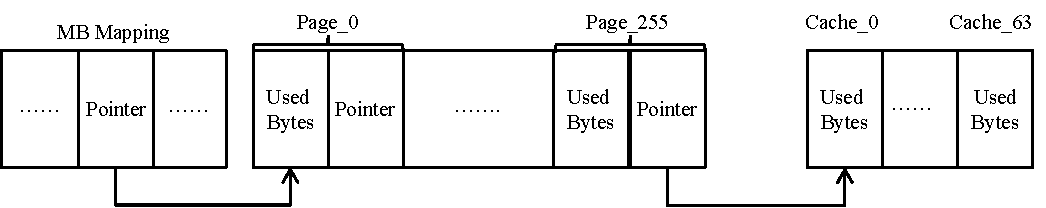
\includegraphics[width=\columnwidth]{figures/lookup}
\caption{Three-level lookup mechanism of \MP{}.\label{fig:lookup}}
\end{figure*}

Note that this design is also efficient in memory consumption. If a range of addresses are not used, then there is no need to allocate physical memory for the corresponding page entries and cache entries. This design is able to adapt to different allocators, where memory mappings of a heap is varied from a few to hundreds of thousands, and these mappings can be scattered along the whole address space of a process. 
%To track valid memory mappings dynamically, \MP{} intercepts memory related system calls inside allocations/deallocations, such as \texttt{sbrk}, \texttt{mmap}, \texttt{munmap}, \texttt{mremap}. 

For false sharing effect, \MP{} focuses on two aspects: the number of cache lines that has false sharing, either active or passive false sharing, and the number of cache contention events on these cache lines. Identifying active and passive false sharing is relatively intuitive based on the definition, by checking the number of threads in each cache line. We employ three-level lookup table as discussed above to store the threads information that are allocated from the same cache line. 
For cache contention events, \MP{} relies on sampled memory accesses. Upon each sampled event, \MP{} checks whether the event is a write access. For each write, \MP{} updates the last thread to write on the corresponding cache line to be the current thread. If the current thread is different from the recorded last thread, \MP{} increments the number of cache contention events. In the end, \MP{} reports the percentage of cache contention on identified cache lines with false sharing issue. 

\MP{} also reports the number of cache contention events on cache lines without active/passive false sharing issues, using the same method. In fact, cache contention events on these cache lines can be caused by internal-object false sharing or true sharing, but they cannot be solved with a different memory allocator. However, the reported data could help understand whether an application is running slow or not. Note that \MP{} is not designed to be false/true sharing detection tool. If \MP{} reports a big cache contention rate, users may resort to specific tools to identify specific issues inside the application~\cite{Sheriff, Predator, DBLP:conf/ppopp/ChabbiWL18}. 
   

\begin{comment}


\subsection{Predicting Performance Impact}
\label{sec:predict}

In order to help users determine whether an allocator is the culprit of the performance issue, \MP{} further predicts the potential performance improvement after switching to  a better allocator. Predicting the performance impact is very complicated, since an application can be affected by multiple factors, such as hardware/software  contention and synchronization. From the point view of an allocator, it can be affected by both cache friendliness and memory management overhead. \MP{} only focuses on the latter one, which provides an lower bound on the potential improvement. Basically, \MP{} replaces the runtime of memory management operations with a standard runtime, and then predicts the reduction of the total runtime.  

For the standard runtime of every memory management operation, \MP{} utilizes the median values collected from a range of applications. Basically, based on our evaluation, the default Linux, TcMalloc, and jemalloc are three best allocators in terms of the performance. Then we choose the best allocator for each application in terms of cycles for each memory management operation, and then select the median value for each operation. Note that there are different choices to choose the standard runtime for every operation, and we only utilizes a simple one to proof the concept. We have thought about that the runtime of a memory management operation can be related with the parallelization and the frequency of allocation. However, it is challenging to build a direct relationship based on our evaluation results. For instance, a serial allocation can also take tens of thousands of cycles. 

To predict the runtime reduction, \MP{} further collects the runtime outside memory management operations with the RDTSC instruction. 
     
	
\end{comment}

\subsection{Adapting To Different Allocators}
\label{sec:understandingallocators}

\MP{} is designed as a general profiler for sequential and BiBOP-style allocators, as described in Section~\ref{sec:allocator}. The primary challenge is to adapt to different allocators. \MP{} interprets a configuration file to identify the differences and unique characteristics of every allocator during its initialization phase, such as the allocator's style (BiBOP-style versus sequential), the sizes of its different classes, and the threshold separating small objects from large objects. Alternatively, this configuration can also be provided manually. \MP{} also provides a pre-run program to automatically determine these details for a given allocator.

In order to identify the style of allocator, the pre-run routine will check whether two subsequent allocations with different sizes (small objects, apparently from different size classes) are satisfied from the same virtual page. If they were, then the allocator is a sequential-style allocator, which is similar to the default Linux allocator. Otherwise, the allocator belongs to a BiBOP-style allocator. 

The second step is to identify the sizes of the various different size classes. The pre-run routine begins by allocating an object of 8 bytes, and continues to allocate additional objects using a stride increase of 8 bytes each time. The determination of size classes depends on the style of the allocator. For BiBOP-style allocators, an allocation with a different size class will be satisfied from a different bag, located in a different page. For sequential allocators, such as the Linux allocator, we employ the \texttt{malloc\_usable\_size} routine to return the bag size for an allocation of the specified size. 

%the distance between two contiguously-allocated objects (with distinct sizes) is utilized to determine the size class. As shown in Fig.~\ref{fig:sizeclass}, if the size of $Obj_1$ and $Obj_2$ is the same, judging from the distance of between two continuous objects, then they belong to the same size class. Otherwise, they belong to different size class, such as $Obj_3$ in the figure. By checking the size of two objects belonging to different objects, we could determine the sizes of different size classes.  
\begin{comment}

\begin{figure}[!ht]
\centering
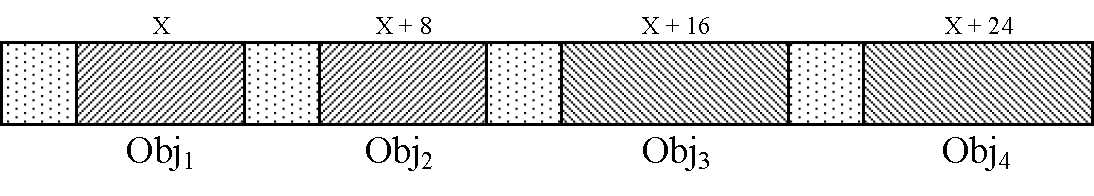
\includegraphics[width=5in]{figures/sequentialclasssize}
\caption{Determining the size class of a sequential allocator by the distance between continuous allocations. \\The boxes with 10\% dotted pattern are the metadata, while the boxes with diagonal stripes\\ are actual heap objects. The number above each box represents the size of the corresponding object. \label{fig:sizeclass}}
\end{figure}
	
\end{comment}

The threshold for big objects are typically detected by checking whether there is an explicit \texttt{mmap} system call upon the allocation request. Typically, most allocators utilize a direct \texttt{mmap} system call to satisfy the allocation of a big object initially. However, this threshold requires manual confirmation.